%!TEX TS-program = pdflatex
% LaTeX-Vorlage zur Erstellung einer Projektarbeit (Dokumentation eines Projekts)
% auf Basis der Vorlage für eine
% Abschlussarbeit in der Fakultät Elektrotechnik, Medien und Informatik an der OTH Amberg-Weiden
% Diese Vorlage entstand im Rahmen des Kurses "LaTeX fürs Studium"
% Aktuelle Version: v0.01
% Stand: 03.06.2023
%
% Changelog:
%
% v0.01: 03.06.2023, Anpassung der Vorlage für Projektarbeiten (article statt report, keine Titelblätter)
%
\documentclass[12pt,oneside]{article}
\usepackage[T1]{fontenc}		% Einstellungen fuer Umlaute usw.
\usepackage[utf8x]{inputenc}
\usepackage[english]{babel}

\usepackage{parskip}			% Einstellungen fuer Absaetze: Abstand statt Einrueckung

\usepackage[a4paper,			% Papierformat A4
	    left=2.5cm,				% linker Rand
	    right=2.5cm,			% rechter Rand
	    top=1.5cm,				% oberer Rand
	    bottom=1.5cm,			% unter Rand
	    marginparsep=5mm,		% Abstand der Randnotizen
	    marginparwidth=10mm, 	% Breite der Randnotizen
	    headheight=7mm,			% Hoehe der Kopfzeile
	    headsep=1.2cm,			% Abstand der Kopfzeile
	    footskip=1.5cm,			% Abstand der Fusszeile
	    includeheadfoot]{geometry}

\usepackage{fancyhdr}						% Konfiguration von Kopf- und Fusszeilen
\pagestyle{fancy}							% Seitenstil 'fancy'
\fancyhf{}									% vorhandene Einstellungen loeschen
\setlength{\headwidth}{\textwidth}			% Kopf- und Fusszeile so breit wie der Haupttext
\fancyfoot[R]{\thepage} 					% Festlegung des Seitenstils: Seitenzahlen in der Fusszeile rechts
\fancyfoot[L]{\IhreArbeit}					% Kapitelnr. und -Bezeichnung in der Fusszeile links
\fancyhead[L]{\IhreGruppe: \IhrVornameEins\ \IhrNachnameEins\ \& \IhrVornameZwei\ \IhrNachnameZwei}	% Vorname und Name in der Kopfzeile links
\renewcommand{\sectionmark}[1]{	    		% Definition der Ausgabe des Kapitels
  \markboth{Abschnitt \thesection. #1}{}}
\renewcommand{\headrulewidth}{0.5pt}		% Trennlinie zwischen Kopfzeile und Haupttext
\renewcommand{\footrulewidth}{0.5pt}		% Trennlinie zwischen Haupttext und Fusszeile
\fancypagestyle{plain}{				     	% Anpassung des Seitenstils 'plain' bei Beginn neuer Kapitel
  \fancyhf{}								% Vorbelegung loeschen
  \fancyfoot[C]{\thepage}					% Seitenzeilen in der Fusszeile mittig
}

\usepackage{amsmath}			% Pakete fuer den Mathematikmodus
\usepackage{amssymb}
\usepackage{amsfonts}
%\usepackage[intlimits]{empheq}

\usepackage[sc]{mathpazo}		% Schriftart Palatino fuer Haupttext und Mathematikmodus
\usepackage{pifont}				% zusaetzliche Symbole

% \usepackage[format=hang,		% Einstellung fuer Bildunterschriften
            % font={footnotesize},
            % labelfont={bf},
            % margin=1cm,
            % aboveskip=5pt,
            % position=bottom]{caption}

\usepackage{graphicx}							% Einbinden von Graphiken
\usepackage[svgnames,cmyk,table,hyperref]{xcolor} 	% Verwendung von Farben

\definecolor{aoenglish}{rgb}{0.0, 0.5, 0.0}
\definecolor{battleshipgrey}{rgb}{0.52, 0.52, 0.51}
\definecolor{cardinal}{rgb}{0.77, 0.12, 0.23}

%\usepackage{tikz}								% Erstellen von Grafiken
%\usetikzlibrary{positioning,arrows,plotmarks} % TikZ-Bibliotheken
%\usepackage{pgfplots}                           % Darstellung von Plots, Funktionen, Graphen usw.

%
% Weitere Pakete
%
\usepackage{listings}			% Darstellung von Quellcode
\lstloadlanguages{[ISO]C++,Java,XML,[LaTeX]TeX}
\lstset{language=C++,
	numbers = none,
	basicstyle = \small\ttfamily,
	keywordstyle = \color{blue},
	commentstyle = \color{battleshipgrey},
	stringstyle = \color{cardinal},
	columns = flexible,
	showstringspaces = false
}
%
\usepackage[square,numbers,sort]{natbib} % Zitationsstil mit Attribut lastchecked
%
%\usepackage[european, siunitx]{circuitikz}	% Darstellung von Schaltungen
%
%\usepackage{enumerate}			% Formatierung nummerierter Listen

% 
% Persoenliche Angaben
% 
\newcommand*{\IhrVornameEins}{Simon}
\newcommand*{\IhrNachnameEins}{Völkl}
\newcommand*{\IhrVornameZwei}{Johannes}
\newcommand*{\IhrNachnameZwei}{Schieder}
\newcommand*{\IhreGruppe}{Group 03}
\newcommand*{\IhrStudiengang}{Artificial Intelligence, Industry-4.0-Informatics}
\newcommand*{\IhreArbeit}{Project Mobile \& Ubiquitous Computing Summer Semester 2026}
\newcommand*{\IhreSchluesselwoerter}{ESP32S3, MQTT, IoT, Tilt Sensor, Node-RED, Wi-Fi} % TODO keywords
\newcommand*{\IhrErstpruefer}{Prof. Dr. Ulrich Schäfer}

\usepackage[bookmarks, raiselinks, pageanchor, % PDF-Einstellungen
            hyperindex, colorlinks,
            citecolor=black, linkcolor=black,
            urlcolor=black, filecolor=black,
            menucolor=black]{hyperref}
\hypersetup{pdftitle={\IhreArbeit},%
            pdfauthor={\IhrVornameEins\ \IhrNachnameEins{} \& \IhrVornameZwei\ \IhrNachnameZwei},%
            pdfsubject={\IhreGruppe},%
            pdfkeywords={\IhreSchluesselwoerter}}

% These packages were proposed by Tobias Bauer in the lecture "LaTeX fürs Studium" in 2026.
% Many adjustments were made to the template for fitting a potential publication of the technical report with Prof. Neumann.
\usepackage[shortlabels]{enumitem} % Verbesserte Einstellungsmöglichkeiten von Listen. Nicht bei Beamer anwendbar
\usepackage{csquotes} % Korrekte Anführungszeichen setzen. Sprachspezifisch möglich. mit \setquotestyle{style} und \enquote{}.
\usepackage[capitalise,nameinlink,noabbrev]{cleveref} % Referenzen besser machen. z.B. mit \cref{}. needs hyperref defined before it.
\usepackage{multirow} % Mehrere Zeilen in eine zusammenfassen. für Spalten einfach \multicolumn benutzen
\usepackage{booktabs} % Hübschere Tabellen mit \top/mid/cmid/bottomrule
\usepackage{minted} % Neuere Bibliothek für Code-Blöcke, mit \begin{listing oder minted}
\usepackage{float}
\usepackage{siunitx}
\usepackage{array}
\usepackage{tabularx}

\begin{document}
\thispagestyle{empty}
%\originalTeX
\begin{center}
	\Large
	Ostbayerische Technische Hochschule Amberg\-/Weiden\\
	Department of Electrical Engineering, Media, and Computer Science\\[.8cm]
	\large \IhrErstpruefer\\[.8cm]
	\Large \IhreArbeit\\[.8cm]
	\large \IhreGruppe: \IhrVornameEins\ \IhrNachnameEins\ \&
	\IhrVornameZwei\ \IhrNachnameZwei\\[.8cm]
	\large Courses of study: \IhrStudiengang\\[.8cm]
	\today\\[2.5cm]
\end{center}

\tableofcontents

\clearpage

\section*{Abstract}
\label{sec:abstract}
% should include keywords.

\section{Introduction}
\label{sec:introduction}

\subsection{Intro}
\label{subsec:intro}
% TODO: write Intro
% Give a brief overview of the project, mission statement, and background.

\subsection{Mission Statement}
\label{subsec:mission_statement}
% TODO: write Mission Statement
% Detail the goal and purpose of the project.

\subsection{Motivation}
\label{subsec:motivation}
% TODO: write Motivation
% Describe why the project is important and the motivation behind it.

\subsection{Document Structure}
\label{subsec:document_structure}
% TODO: write Document Structure
% Give an overview of how the rest of the document is structured.

\section{Related Work}
\label{sec:related_work}
% TODO: write Related Work
% Discuss existing similar projects, solutions and relevant literature.

\section{Project Management}
\label{sec:project_management}

\subsection{SMART}
\label{subsec:smart}
% TODO: write SMART
% Outline the SMART goals (Specific, Measurable, Achievable, Relevant, Time-bound).

\subsection{User Stories (Requirements)}
\label{subsec:user_stories}
% TODO: write User Stories (Requirements)
% Detail the requirements and user stories for the project.

\subsection{MVP}
\label{subsec:mvp}
% TODO: write MVP
% Describe the Minimum Viable Product.

\subsection{Extensions}
\label{subsec:extensions}
% TODO: write Extensions
% Discuss potential extensions or features beyond the MVP.

\subsection{Task Distribution}
\label{subsec:task_distribution}
% TODO: write Task Distribution
% Provide a breakdown of tasks among group members and list guidelines (PRs, Code Coverage, Git).

\section{Technical Concept}
\label{sec:technical_concept}

\subsection{High-Level Architecture}
\label{subsec:high_level_architecture}
% TODO: write High-Level Architecture
% Explain the high-level architecture with a diagram.

\subsection{Components}
\label{subsec:components_concept}
% TODO: write Components
% Give an overview of the main components (Hardware, Node-RED, Android).

\section{Hardware}
\label{sec:hardware}

\subsection{Components (ESP32) in Detail}
\label{subsec:components_hardware}
% TODO: write Components (ESP32) in Detail
% Describe the hardware components in detail, especially the ESP32.

\subsection{Sensor Data Acquisition}
\label{subsec:sensor_data_acquisition}
% TODO: write Sensor Data Acquisition
% Detail the data acquisition from the sensors and filtering.

\subsection{Physics Simulation}
\label{subsec:physics_simulation}
% TODO: write Physics Simulation
% Explain the physics simulation with its mathematical formulas.

\subsection{Display}
\label{subsec:display}
% TODO: write Display
% Detail the display logic and game mechanics with screenshots.

\subsection{MQTT Topics \& Payloads}
\label{subsec:mqtt_topics}
% TODO: write MQTT Topics & Payloads
% List the MQTT topics used and their respective JSON payloads.

\section{Node-RED}
\label{sec:nodered}

\subsection{Workflow}
\label{subsec:workflow}
% TODO: write Workflow
% Explain the Node-RED workflow and add a screenshot.

\subsection{Dashboard \& User Input}
\label{subsec:dashboard_nodered}
% TODO: write Dashboard & User Input
% Detail the Node-RED dashboard logic and forms with a screenshot.

\section{Android App}
\label{sec:android_app}

\subsection{Software Components, Classes, Views}
\label{subsec:software_android}
% TODO: write Software Components, Classes, Views
% Document the Android app's architecture, key classes and UI views.

\subsection{Dashboard \& User Input}
\label{subsec:dashboard_android}
% TODO: write Dashboard & User Input
% Explain the dashboard and user input on Android with a screenshot.

\section{Evaluation}
\label{sec:evaluation}

\subsection{Problems \& Solutions}
\label{subsec:problems_solutions}
% TODO: write Problems & Solutions
% Discuss any difficulties encountered and how they were solved.

\subsection{Code Coverage}
\label{subsec:code_coverage}
% TODO: write Code Coverage
% Report on the code coverage of the tests.

\subsection{Cost Estimation}
\label{subsec:cost_estimation}
% TODO: write Cost Estimation
% Provide a cost estimation for the project hardware and setup.

\section{Summary}
\label{sec:summary}

\subsection{Summary \& Future Work}
\label{subsec:summary_future_work}
% TODO: write Summary & Future Work
% Summarize the project and outline ideas for future improvements.

\appendix

\section{Prompts}
\label{sec:prompts}
% TODO: write Prompts
% Attach AI tool prompts used during the development phase.

\section{ESP32 Code}
\label{sec:esp32_code}
% TODO: write ESP32 Code
% Include relevant parts of the ESP32 implementation source code.

% -------------------------
% \begin{figure}[h]
% 	\centering
% 	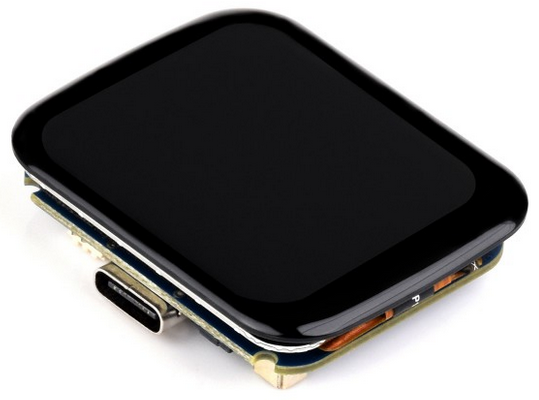
\includegraphics[width=0.3\linewidth]{imgFirstPage.png}
% 	\caption[Waveshare ESP32-S3]{Waveshare ESP32-S3 1.69inch Touch Display Development Board, 240×280 Pixels (Quelle: waveshare.com)}
% 	\label{fig:waveshare}
% \end{figure}
% 
% \begin{lstlisting}[language=C++]
% void setup() {
%   Serial.begin(115200);
%   // gibt etwas aus ueber die serielle Leitung:
%   Serial.println("Hallo ESP");
% }
% \end{lstlisting}
% 
% \begin{lstlisting}[language=Java]
% /**
% * Ein Hallo-Welt-Programm in Java.
% * Dies ist ein Javadoc-Kommentar.
% *
% * @author Ulrich Schaefer
% * @version 1.0
% */
% public class HalloWelt {
% /**
% * Main-Methode
% *
% * @param args Kommandozeilenparameter
% * @return Rueckgabewert
% */
%   public static int main(String[] args) {
%     System.out.println("Hallo Welt!");
%   }
% } // Ende der Java-Klasse HalloWelt
% \end{lstlisting}
% 
% \begin{lstlisting}[language=XML]
% <spitze>
%   <!-- Kommentar in XML -->
%   <klammer wert="auf"/>
% </spitze>
% \end{lstlisting}
% -------------------------

% - bei Bedarf diesen Seitenumbruch entfernen
\clearpage

\phantomsection
\addcontentsline{toc}{section}{References}
\bibliographystyle{natdin}
\bibliography{references}

%\include{anhang} % zum Beispiel hier die ChatGPT-Chatprotokolle einbinden (oder als extra-Datei)

\end{document}
